\documentclass[a4paper,10pt]{article} % добавить leqno в [] для нумерации слева
\usepackage[a4paper,top=1.3cm,bottom=2cm,left=1.5cm,right=1.5cm,marginparwidth=0.70cm]{geometry}

\usepackage[warn]{mathtext}
\usepackage[T2A]{fontenc}
\usepackage[utf8]{inputenc} 
\usepackage[english, russian]{babel}
\usepackage{hyperref}
\hypersetup{
    colorlinks=true,
    linkcolor=blue,
    filecolor=magenta,      
    urlcolor=cyan,
    pdftitle={Overleaf Example},
    pdfpagemode=FullScreen,
}

\usepackage[table,xcdraw]{xcolor}

\usepackage{indentfirst} %tabutation

\usepackage{amsmath, amsfonts, amssymb, amsthm, mathtools, mathtext} 

\usepackage{graphicx}

\usepackage{tabularx}

\usepackage{graphicx}%Вставка картинок правильная

%%% Дополнительная работа с математикой
\usepackage{amsmath,amsfonts,amssymb,amsthm,mathtools} % AMS

%%% Заголовок
\date{\today}

\begin{document}

\begin{titlepage}
	\begin{center}
		{\large МОСКОВСКИЙ ФИЗИКО-ТЕХНИЧЕСКИЙ ИНСТИТУТ (НАЦИОНАЛЬНЫЙ ИССЛЕДОВАТЕЛЬСКИЙ УНИВЕРСИТЕТ)}
	\end{center}
	\begin{center}
		{\large Физтех-школа радиотехники и компьютерных технологий}
	\end{center}
	
	
	\vspace{4cm}
	{\huge
		\begin{center}
			{\bf Лабораторная работа № 2.4.1}\\
			 Определение теплоты испарения жидкости.
		\end{center}
	}
	\vspace{3cm}
	\begin{flushright}
		{\LARGE Авторы:\\ Устюжанина Мария Алексеевна,

		Федорищева Анастасия Анатольевна, 

		Романов Александр Викторович, 

		Пархоцевич Иван Николаевич\\
			\vspace{0.3cm}
			Б01-107}
	\end{flushright}
	\vspace{4.5 cm}
	\begin{center}
		Долгопрудный 2022

	\vspace{1 cm}

		 *В данном исследовании был изучен жизненно важно очень необходимый, волнующий всех вопрос. Надеемся, что наши читатели будут крайне благодарны нам за столь ценные выводы, которые они сделают после прочтения. 
		 Целью нашей работы является вдохновение читателей!

	\end{center}
\end{titlepage}

\section{Введение}

Вопросам, связанным с исследованием испарения жидкости, было посвящено большое количество исследований, что связано с практической важностью этого направления. 

Испарение жидкости играет ведущую роль в отраслях промышленности. Именно поэтому продолжение исследований особенностей его протекания является актуальным и по сей день как с теоретической, так и с практической точки зрения.

\textbf{Цель работы:}

1) Измерение давления насыщенного пара жидкости при разной температуре; 

2) Вычисление по полученным данным
теплоты испарения с помощью уравнения Клапейрона–Клаузиуса.

\textbf{Используемое оборудование:}

Термостат; герметический сосуд, заполненный исследуемой жидкостью; отсчетный микроскоп.

\section{Основная часть}

Одно и то же вещество при одних и тех же температуре и давлении может находиться в газообразном, жидком и твердом состояниях, причем эти состояния (фазы) могут существовать одновременно, находясь в контакте друг с другом.
 Эти состояния отличаются своими физическими свойствами. Переход вещества из одной фазы в другую называется фазовым переходом или фазовым превращением. Испарение — переход жидкости в пар, являются примером фазовых переходов. 

В уравнении Ван-дер-Ваальса жидкость может находиться в равновесии со своим паром. Это равновесие с паром, который в таком случае называется насыщенным паром, устанавливается само собой, если жидкость находится в закрытом сосуде.
Процесс установления равновесия сводится к тому, что с поверхности жидкости вылетает часть молекул, образуя над жидкостью пар. Для выхода из жидкости испаряющиеся молекулы должны преодолеть силы притяжения со стороны оставшихся молекул, т. е. совершить работу против этих сил. Кроме того, должна быть совершена работа против внешнего давления р уже
образовавшегося пара, равная $p\Delta V$, где $\Delta V$ —изменение объема,
занимаемого данным количеством молекул при переходе из жидкости в пар. Вся эта работа может быть совершена только за счет кинетической энергии теплового движения молекул. Очевидно, что не все молекулы способны совершить эту работу, а только те из них, которые обладают достаточной для этого кинетической энергией. Поэтому переход части молекул в пар приводит к обеднению жидкости быстрыми молекулами,т. е. к ее охлаждению.

Давление насыщенного пара какого-либо вещества зависит от температуры и не зависит от объема пара, а также от давления других газообразных примесей, если они трудно растворимы в данной жидкости или в данном твердом теле.

Для вывода соотношения между температурой и давлением насыщенного пара жидкости обычно рассматривают равновесный переход одного моля вещества из одной фазы (1) в дpyгyю (2) при постоянных давлении и температуре. Изобарные потенциалы ($G_i$) единицы массы чистого вещества в двух фазах однокомпонентной системы, находящихся в равновесии, при условии, что
число молей компонента в жидкой и паровой фазах равны единице, равны между собой

\[G_1 = G_2\]
\[dG_1 = dG_2\]

Уравнение в дифференциальной форме для  изобарных потенциалов для одного моля в фазах 1 и 2 принимает следующий вид:

\[dG_1 = V_1dp - S_1dT\]
\[dG_2 = V_2dp - S_2dT\]

Вычитая нижнее уравнение из верхнего, получим:
\[dG_2 - dG_1 = (V_2-V_1)dp - (S_2-S_1)dT \]

Следовательно, $(V_2-V_1)dp - (S_2 - S_1)dT = 0$.
Получим уравнение:

\[\frac{dp}{dT} = \frac{S_2 - S_1}{V_2-V_1}\]

Известно, что:

\[S_2 - S_1 = \frac{L}{T}\]

где L - теплота испарения жидкости.

В уравнении Ван-дер-Ваальса:
\[(P+\frac{a}{V^2})(V-b) = RT\]

пренебрежем величинами $b$ и $\frac{a}{V^2}$. Тогда получим: 

\[ V = \frac{RT}{P} \]

В итоге для удельной теплоты испарения: 
\[L = \frac{RT^2}{P}\frac{dP}{dT} = -R\frac{d(ln(P))}{d(1/T)}\]



Применяемый нами диагностический метод является классическим и описан в источнике Гладун A.Д. Лабораторный практикум по общей физики. Т.I. Термодинамика и молекулярная физика. стр 234-235.



\medskip

\textbf{Экспериментальная установка.}
Установка включает термостат A, экспериментальный прибор B и отсчетный микроскоп C. Экспериментальный прибор B представляет собой емкость 12, заполненную водой. В нее погружен запаянный прибор 13 с исследуемой жидкостью 14. Перед заполнением исследуемой жидкости воздух
из запаянного прибора был удален, так что над жидкостью находится только её насыщенный пар.
Давление пара определяется по ртутному манометру 15, соединенному с емкостью 13.

\begin{figure}[h]
	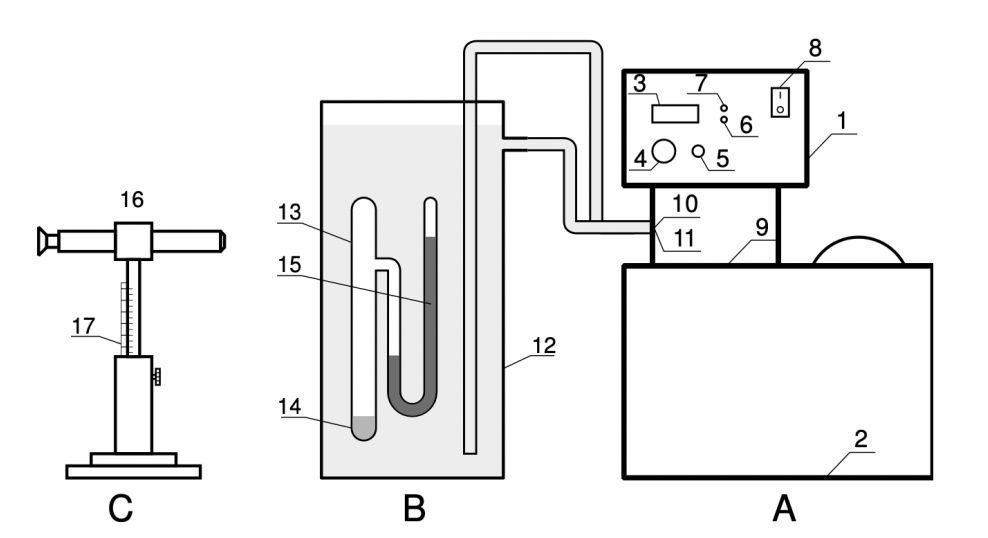
\includegraphics[scale=0.8]{Picture1}}
	\caption{Схема установки для определения теплоты испарения}
\end{figure}

	
\section {Обработка результатов}
\textbf{При измерении давления и температуры во время нагревания термостата были получены следующие данные:}\\

$$
\begin{tabular}{|c|c|c|c|c|c|c|c|c|c|c|c|c|c|}
\hline
\multicolumn{14}{|c|}{Данные для графика при нагреве}\\
\hline
$T, K$&294.2&297.2&299.2&301.2&303.2&305.2&307.2&309.2&311.2&313.2&315.2&317.2&318.2\\\hline
$P, Pa$&2584&3128&3400&3808&4216&4760&5168&5848&6664&7072&8024&8840&9384\\\hline
\end{tabular}
$$


Получена экспоненциальная зависимость: \\


\begin{center}
	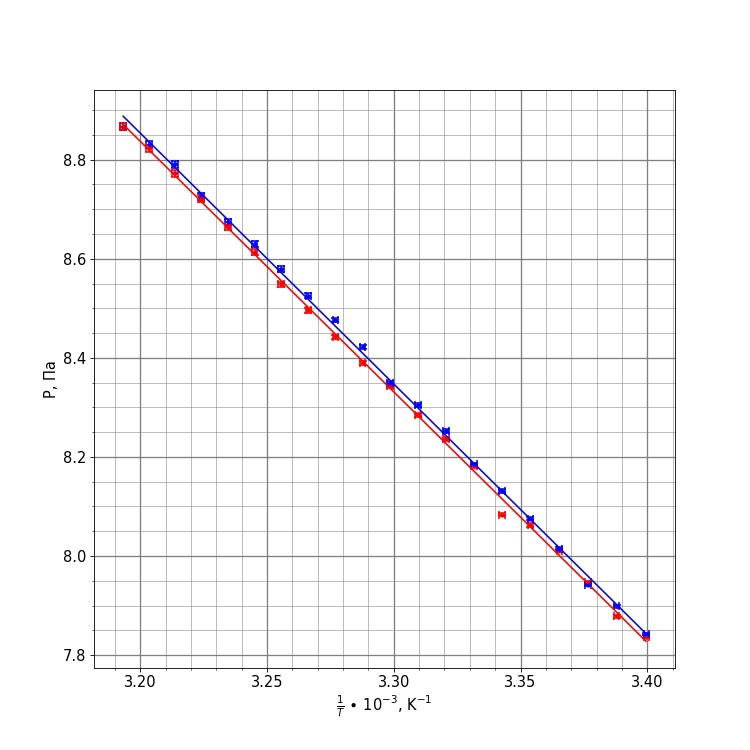
\includegraphics[width=0.8\textwidth]{graph1.png}
\end{center}

Зависимость: $P = e^{0.053\cdot T}$, погрешность коэффициента экспоненты равна $4.7\cdot 10^{-4}$ \\




График $\ln(P)$ от $\frac{1}{T}$:\\
$$
\begin{tabular}{|c|c|c|c|c|c|c|c|c|c|c|c|c|c|}
\hline
\multicolumn{14}{|c|}{При нагреве}\\
\hline
$1/T, 1e-3 K^-1$&3.399&3.387&3.365&3.342&3.320&3.298&3.276&3.255&3.234&3.213&3.192&3.172&3.153\\\hline
$ln(\P)$&7.857&8.048&8.132&8.245&8.347&8.468&8.550&8.674&8.804&8.864&8.990&9.087&9.147\\\hline
\end{tabular}
$$



\begin{center}
	\includegraphics[width=0.75\textwidth]{graph3.png}
\end{center}

Полученная зависимость вида $y = (kx + b)$: \
$ln(P) = -4994\cdot \frac{1}{T} + 24.8,\ \sigma_k = 46.56, \ \sigma_b = 0.0037$\\
Подставляя угловой коэффициент в формулу:
$$L = -R\frac{d(lnP)}{d(1/T)}$$
Получим значение удельной теплоты парообразования: $L = 41500 \pm 389$ Дж/моль $= 2.3 \pm 0.021$ $10^{6}$ Дж/кг.\\

\medskip

\

\

\newline
\textbf{Во время охлаждения:}\\


\begin{center}
\begin{tabular}{|c|c|c|c|c|c|c|c|c|c|c|c|c|}
\hline
\multicolumn{13}{|c|}{Данные для графика при охлаждении}\\
\hline
$T, K$&318.2&317.2&315.2&313.2&311.2&309.2&307.2&305.2&303.2&301.2&299.2&297.2\\\hline
$P, Pa$&9384&9248&8296&7548&6800&5984&5304&4964&4420&4080&3536&3196\\\hline
\end{tabular}
\end{center}

Получена экспоненциальная зависимость: \\

\begin{center}
	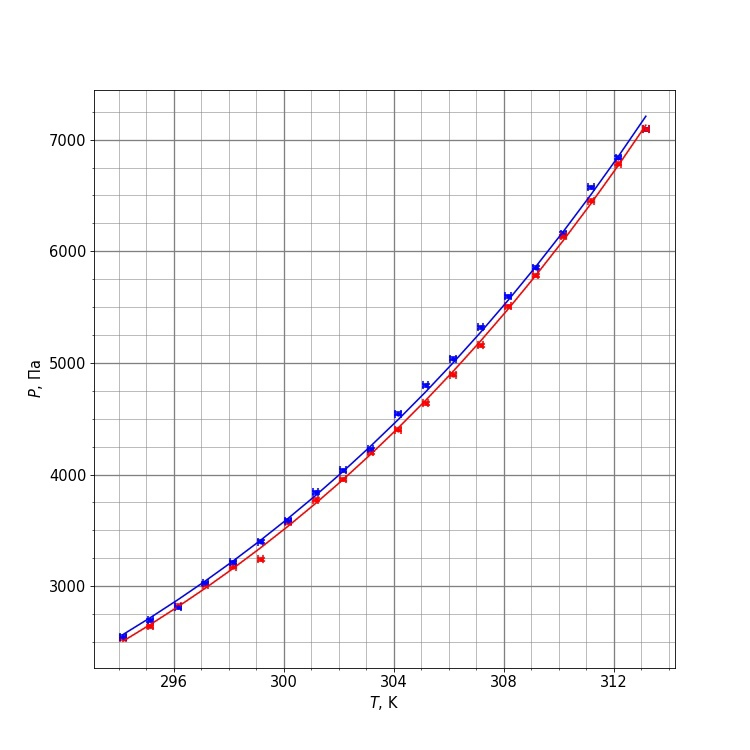
\includegraphics[width=0.8\textwidth]{graph2.png}
\end{center}

Зависимость: $y = exp(0.052\cdot T)$, погрешность коэффициента экспоненты равна $6.9\cdot 10^{-4}$\\
Логарифмический график при остывании:\\

\begin{tabular}{|c|c|c|c|c|c|c|c|c|c|c|c|c|c|}
\hline
\multicolumn{14}{|c|}{При охлаждении}\\
\hline
$1/T, 1e-3 K^-1$&3.399&3.387&3.365&3.342&3.320&3.298&3.276&3.255&3.234&3.213&3.192&3.172&3.153\\\hline
$ln(\Delta P)$&9.09&9.147&9.132&9.023&8.929&8.824&8.696&8.576&8.509&8.393&8.313&8.170&8.069\\\hline
\end{tabular}\\

Получена линейная зависимость: \\

\begin{center}
	\includegraphics[width=0.8\textwidth]{graph4.png}
\end{center}


Полученная зависимость (вида $y = kx + b$): $ln(P) = -4902\cdot \frac{1}{T} + 24.56, \sigma_k = 63.15, \sigma_b = 0.0046$\\


Подставляя угловой коэффициент в формулу:

$$L = -R\frac{d(lnP)}{d(1/T)}$$
Получим значение удельной теплоты парообразования: $L = 40735 \pm 524$ Дж/моль $= 2.26 \pm 0.029$ $10^6$Дж/кг.\\




\section{Заключение}

	При помощи термостата в  сосуде поддерживается необходимая температура исследуемой жидкости. К сосуду герметично припаян U-образный капилляр с запаянным концом. Внутри капилляра находится ртуть. При нагревании жидкости давление пара возрастает, за счет чего появляется различие в уровнях ртути. По разности уровней и определяется изменение давлений. 

	В работе получена зависимость давления насыщенных паров при разных температурах. По полученным данным найдена удельная теплота парообразования воды. $L_{up} = 41500 \pm 389 \frac{Дж}{моль}$ и $L_{down} = 40735 \pm 524 \frac{Дж}{моль}$. Сравнивая эти результаты с табличным $L_{табл} = 41630 \frac{Дж}{моль}$ получаем, что значение при нагреве термостата совпадает с табличным в пределах погрешности, а в процессе охлаждения отличаются примерно на две погрешности, что однако также является довольно точным приближением. Разницу в этих значения можно объяснить неидеальностью экспериментальной установки и действий экспериментатора.

	Полученные результаты могут использоваться для проектирования бытовых приборов таких как чайники, скороварки, увлажнители воздуха и др. Так же для отслеживания испарений ценных ресурсов таких как нефть, различное топливо и др. 

	В дальнейшем можно исследовать давление пара в большем диапазоне температур или испаряемость других более маслянистых жидкостей (нефть,   подсолнечное масло) или топлива (бензин, дизель), а также оценить их давление на топливную систему.

\section{Список литературы}
	\begin{enumerate}
		\item Сивухин Д.В. Общий курс физики. Т. II. Термодинамика и молекулярная физика.
		\item Гладун A.Д. Лабораторный практикум по общей физики. Т.I. Термодинамика и молекулярная физика.
		\item Кикоин А.К., Кикоин И.К. Общий курс физики. Молекулярная физика. Издание второе, переработанное - М.: 1976. - 480 с.
		\item \url{https://cyberleninka.ru/article/n/issledovanie-temperaturnoy-zavisimosti-skorosti-ispareniya-zhidkostey-so-svobodnoy-poverhnosti-i-skorosti-kipeniya-zhidkosti-na/viewer}
		\item \url{https://www.gubkin.ru/faculty/chemical_and_environmental/chairs_and_departments/physical_and_colloid_chemistry/files/fazovoye_ravnovesiye.pdf}

	\end{enumerate}





\end{document}
